\section{Rectificatifs du rapport de spécifications fonctionnelles}
\label{sec:rect}

\subsection{Architecture générale}
La {\sc Figure} \ref{fig:archiPrevue} illustre l'architecture générale imaginée lors du rapport de spécifications fonctionnelles. Suite à des contraintes techniques, notamment dues au fait qu'un programme Java est difficilement contrôlable depuis un programme C\#, l'architecture a été revue pour correspondre à celle présentée à la {\sc Figure} \ref{fig:archiReelle}. 

ADTool ne fait finalement pas partie intégrante de Glasir, mais est lancé en tant que simple \og viewer \fg{} d'ADTree. En effet, il est impossible, depuis Glasir, de détecter des modifications faites dans ADTool, comme par exemple la modification d'une valuation à l'une des feuilles de l'ADTree. Par conséquent, la décision fut prise de désactiver toutes les fonctions d'édition dans ADTool lorsque Glasir se lance, donnant ainsi à ADTool un mode spécial batpisé \og viewmode \fg{} dans lequel l'utilisateur ne peut que visualiser un ADTree, sans pouvoir le modifier.

		\begin{figure}[H]
            \centering
                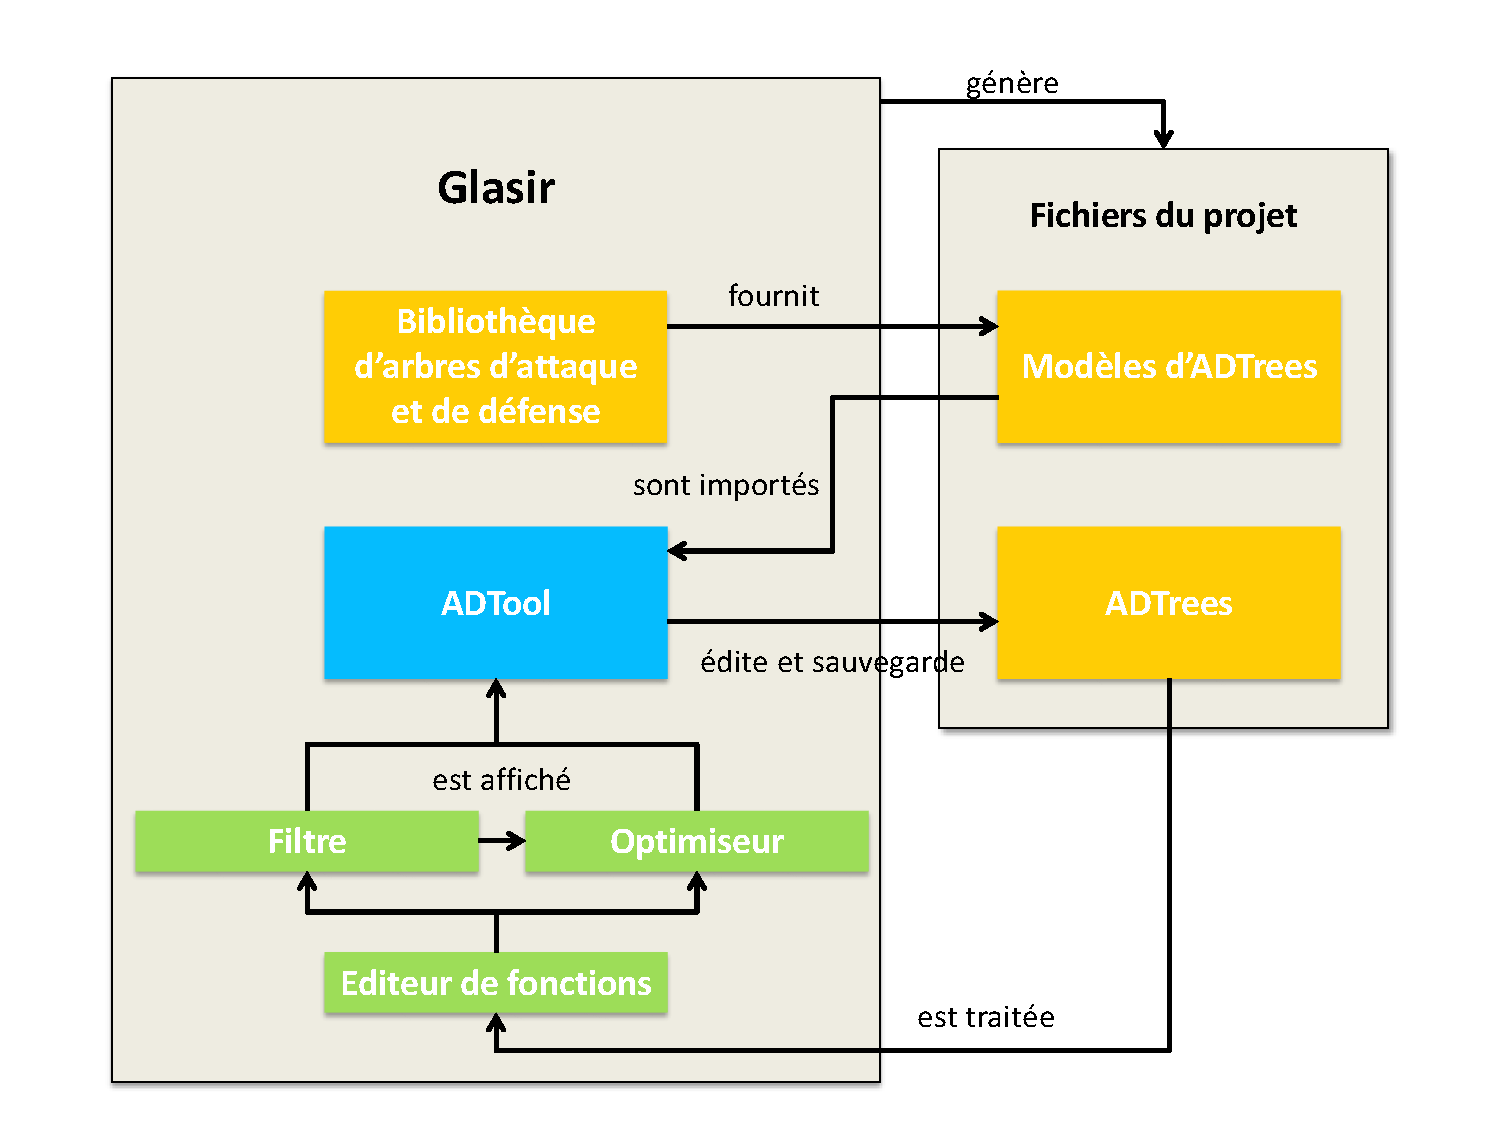
\includegraphics[width=0.8\textwidth]{figure/archiGlasir.pdf}
            \caption{Architecture initialement prévue.}
            \label{fig:archiPrevue}
        \end{figure}
	
        
        \begin{figure}[H]
            \centering
                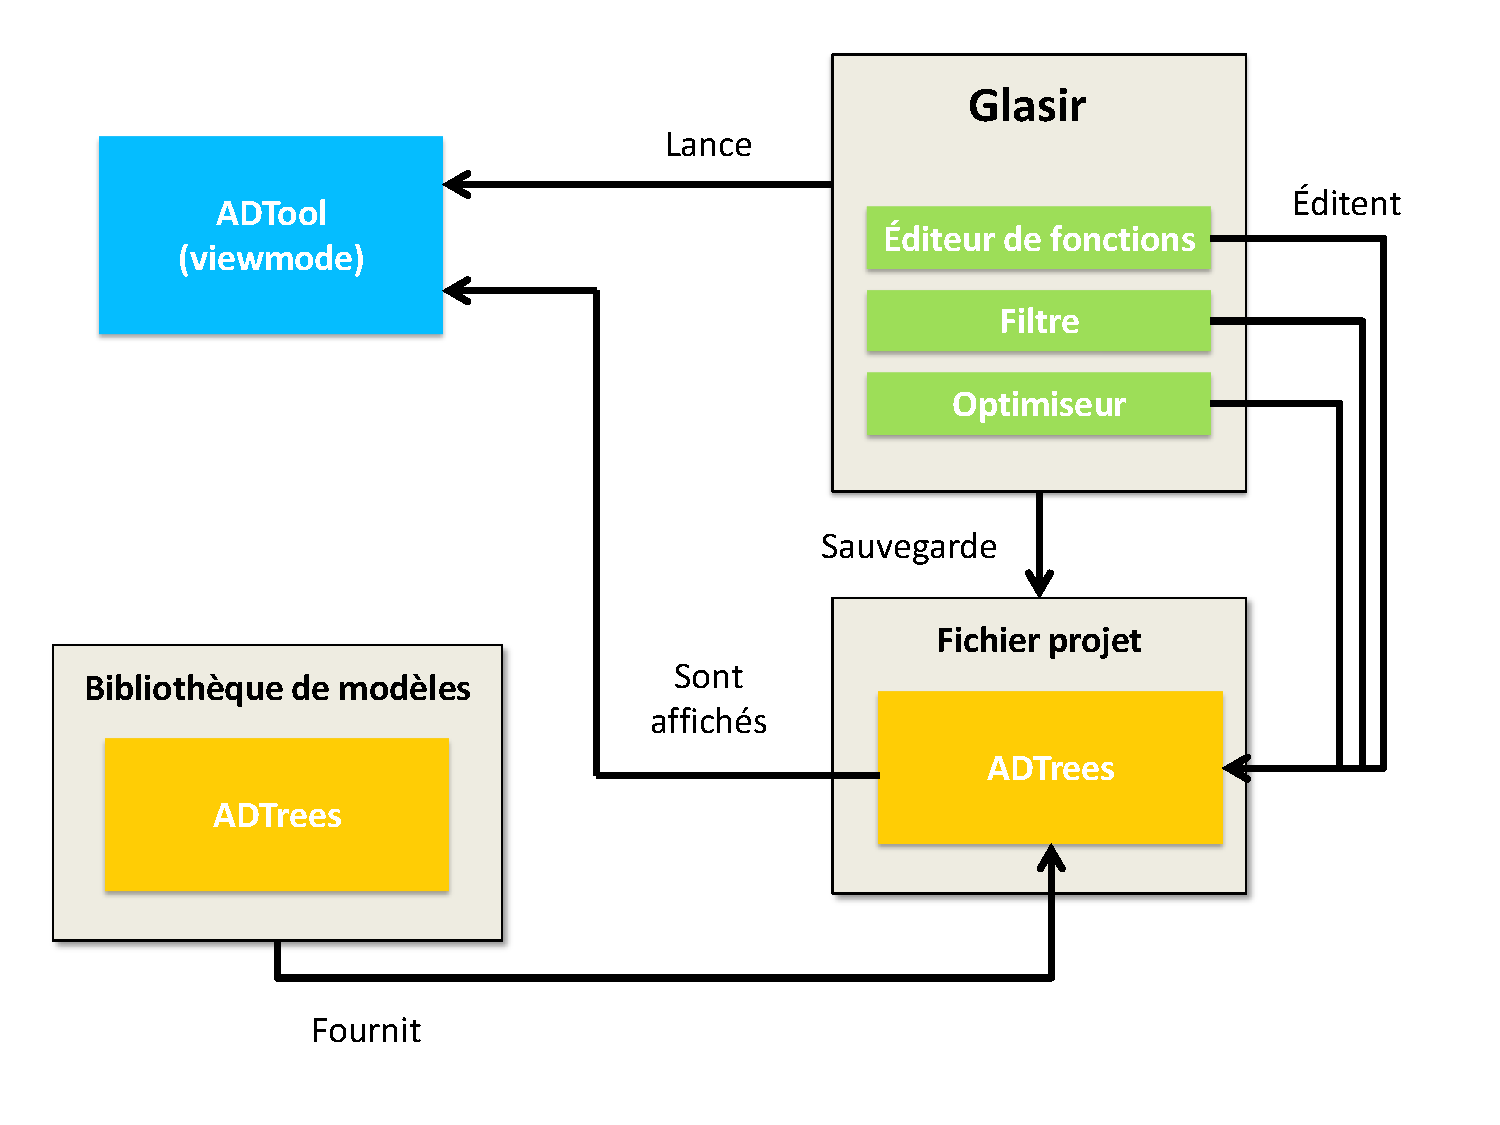
\includegraphics[width=0.8\textwidth]{figure/archiReelle.pdf}
            \caption{Architecture réelle.}
            \label{fig:archiReelle}
        \end{figure}
        
        
\subsection{Algorithme de l'Éditeur de fonction}
	L'algorithme.

\subsection{Algorithme du Filtre}
 	L'algorithme.

\subsection{Algorithme de l'Optimiseur}
	L'algorithme.
        

\newpage
\section{Rectificatifs du rapport de conception}
\label{sec:rectConc}

La {\sc Figure} \ref{fig:copypastePrevu} illustre l'implémentation du copy-paste imaginée lors du rapport de conception. Pour des raisons techniques, l'implémentation du copy-paste est telle qu'indiqué sur la {\sc Figure} \ref{fig:copypasteReel}. De même, la {\sc Figure} \ref{fig:ctrlzPrevu} illustre l'implémentation du ctrl-z imaginée lors du rapport de conception, tandis la {\sc Figure} \ref{fig:ctrlzReel} indique son implémentation réelle.

	\subsection{Affichage multiple des paramètres}

	\subsection{Couper-copier-coller}
		\begin{figure}
            \centering
                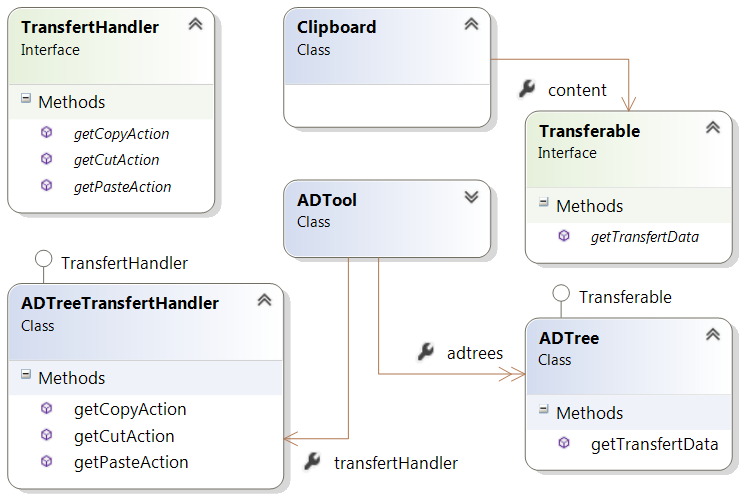
\includegraphics[width=0.8\textwidth]{figure/copiercoller.png}
            \caption{Diagramme de classe prévu pour le couper-copier-coller.}
            \label{fig:copypastePrevu}
        \end{figure}
        
        \begin{figure}
            \centering
                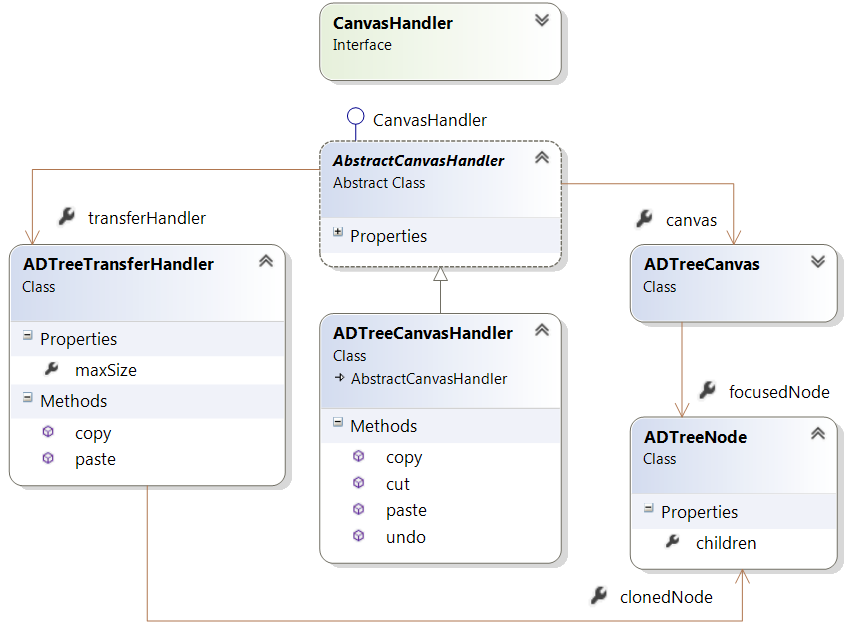
\includegraphics[width=0.8\textwidth]{figure/copiercollerReel.png}
            \caption{Diagramme de classe réel pour le couper-copier-coller.}
            \label{fig:copypasteReel}
        \end{figure}
       
	\subsection{Annulation des dernières actions}
		Blablabla bullshit bullshit
        \begin{figure}
            \centering
                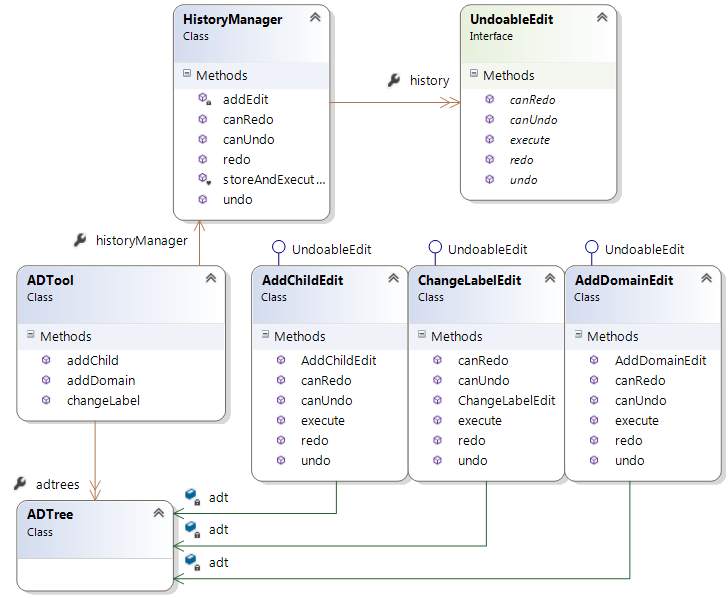
\includegraphics[width=0.8\textwidth]{figure/ctrlz.png}
            \caption{Diagramme de classe prévu pour l'annulation des dernières actions.}
            \label{fig:ctrlzPrevu}
        \end{figure}
        
        \begin{figure}
            \centering
                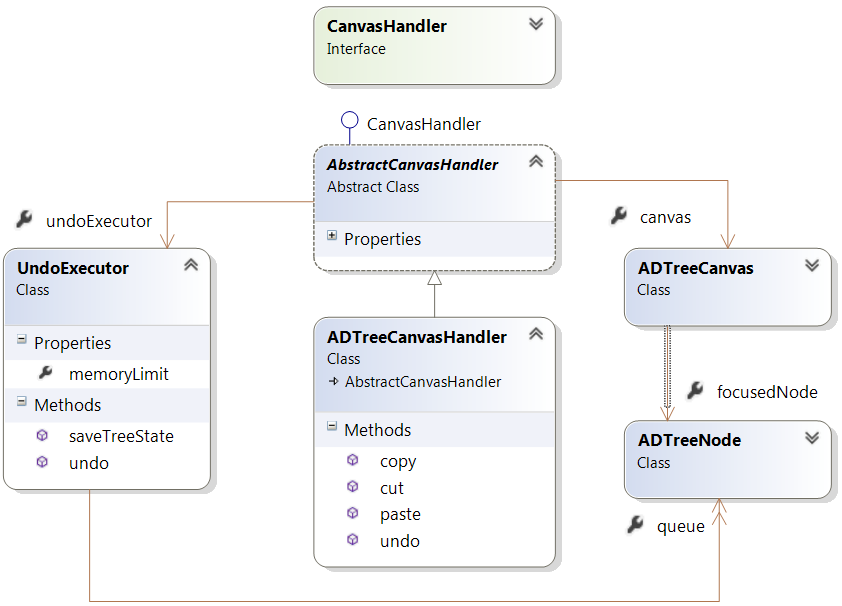
\includegraphics[width=0.8\textwidth]{figure/ctrlzReel.png}
            \caption{Diagramme de classe réel pour l'annulation des dernières actions.}
            \label{fig:ctrlzReel}
        \end{figure}

	\subsection{Bibliothèque de modèles}
		La bibliothèque de modèles n'a finalement pas été implémentée.
		\begin{figure}
            \centering
                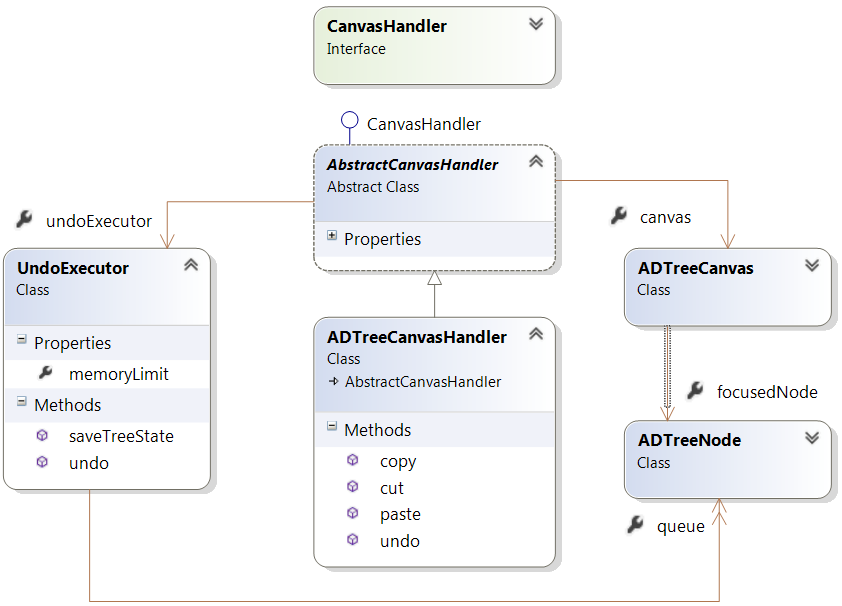
\includegraphics[width=0.8\textwidth]{figure/ctrlzReel.png}
            \caption{Diagramme de classe prévu pour la bibliothèque de modèles.}
            \label{fig:library}
        \end{figure}